% Created by tikzDevice version 0.12 on 2020-03-31 13:55:27
% !TEX encoding = UTF-8 Unicode
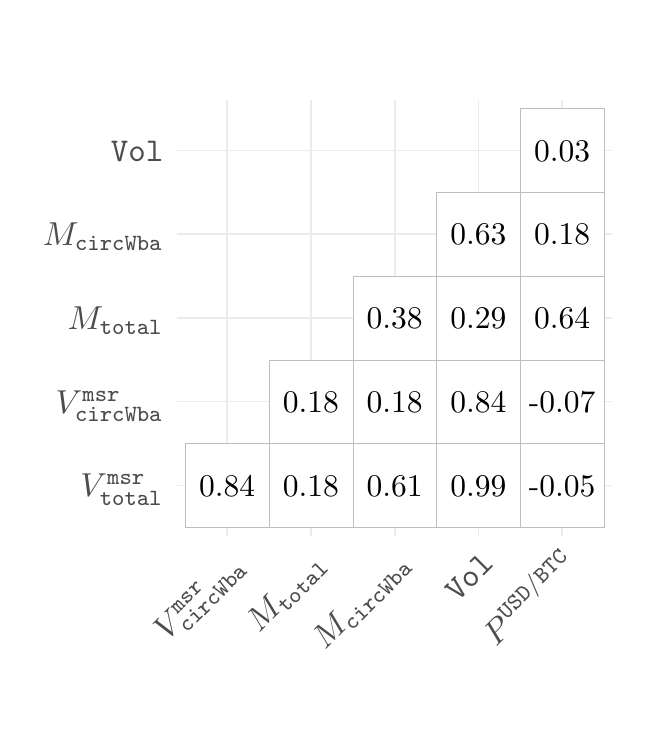
\begin{tikzpicture}[x=1pt,y=1pt]
\definecolor{fillColor}{RGB}{255,255,255}
\path[use as bounding box,fill=fillColor,fill opacity=0.00] (0,0) rectangle (216.81,252.94);
\begin{scope}
\path[clip] ( 53.93, 69.38) rectangle (211.31,226.76);
\definecolor{drawColor}{gray}{0.92}

\path[draw=drawColor,line width= 0.6pt,line join=round] ( 53.93, 87.54) --
	(211.31, 87.54);

\path[draw=drawColor,line width= 0.6pt,line join=round] ( 53.93,117.80) --
	(211.31,117.80);

\path[draw=drawColor,line width= 0.6pt,line join=round] ( 53.93,148.07) --
	(211.31,148.07);

\path[draw=drawColor,line width= 0.6pt,line join=round] ( 53.93,178.33) --
	(211.31,178.33);

\path[draw=drawColor,line width= 0.6pt,line join=round] ( 53.93,208.60) --
	(211.31,208.60);

\path[draw=drawColor,line width= 0.6pt,line join=round] ( 72.09, 69.38) --
	( 72.09,226.76);

\path[draw=drawColor,line width= 0.6pt,line join=round] (102.35, 69.38) --
	(102.35,226.76);

\path[draw=drawColor,line width= 0.6pt,line join=round] (132.62, 69.38) --
	(132.62,226.76);

\path[draw=drawColor,line width= 0.6pt,line join=round] (162.89, 69.38) --
	(162.89,226.76);

\path[draw=drawColor,line width= 0.6pt,line join=round] (193.15, 69.38) --
	(193.15,226.76);
\definecolor{drawColor}{RGB}{190,190,190}
\definecolor{fillColor}{RGB}{255,255,255}

\path[draw=drawColor,line width= 0.1pt,line cap=rect,fill=fillColor] ( 56.96, 72.40) rectangle ( 87.22,102.67);

\path[draw=drawColor,line width= 0.1pt,line cap=rect,fill=fillColor] ( 87.22, 72.40) rectangle (117.49,102.67);

\path[draw=drawColor,line width= 0.1pt,line cap=rect,fill=fillColor] (117.49, 72.40) rectangle (147.75,102.67);

\path[draw=drawColor,line width= 0.1pt,line cap=rect,fill=fillColor] (147.75, 72.40) rectangle (178.02,102.67);

\path[draw=drawColor,line width= 0.1pt,line cap=rect,fill=fillColor] (178.02, 72.40) rectangle (208.28,102.67);

\path[draw=drawColor,line width= 0.1pt,line cap=rect,fill=fillColor] ( 87.22,102.67) rectangle (117.49,132.93);

\path[draw=drawColor,line width= 0.1pt,line cap=rect,fill=fillColor] (117.49,102.67) rectangle (147.75,132.93);

\path[draw=drawColor,line width= 0.1pt,line cap=rect,fill=fillColor] (147.75,102.67) rectangle (178.02,132.93);

\path[draw=drawColor,line width= 0.1pt,line cap=rect,fill=fillColor] (178.02,102.67) rectangle (208.28,132.93);

\path[draw=drawColor,line width= 0.1pt,line cap=rect,fill=fillColor] (117.49,132.93) rectangle (147.75,163.20);

\path[draw=drawColor,line width= 0.1pt,line cap=rect,fill=fillColor] (147.75,132.93) rectangle (178.02,163.20);

\path[draw=drawColor,line width= 0.1pt,line cap=rect,fill=fillColor] (178.02,132.93) rectangle (208.28,163.20);

\path[draw=drawColor,line width= 0.1pt,line cap=rect,fill=fillColor] (147.75,163.20) rectangle (178.02,193.46);

\path[draw=drawColor,line width= 0.1pt,line cap=rect,fill=fillColor] (178.02,163.20) rectangle (208.28,193.46);

\path[draw=drawColor,line width= 0.1pt,line cap=rect,fill=fillColor] (178.02,193.46) rectangle (208.28,223.73);
\definecolor{drawColor}{RGB}{0,0,0}

\node[text=drawColor,anchor=base,inner sep=0pt, outer sep=0pt, scale=  1.14] at ( 72.09, 83.62) {0.84};

\node[text=drawColor,anchor=base,inner sep=0pt, outer sep=0pt, scale=  1.14] at (102.35, 83.62) {0.18};

\node[text=drawColor,anchor=base,inner sep=0pt, outer sep=0pt, scale=  1.14] at (132.62, 83.62) {0.61};

\node[text=drawColor,anchor=base,inner sep=0pt, outer sep=0pt, scale=  1.14] at (162.89, 83.62) {0.99};

\node[text=drawColor,anchor=base,inner sep=0pt, outer sep=0pt, scale=  1.14] at (193.15, 83.62) {-0.05};

\node[text=drawColor,anchor=base,inner sep=0pt, outer sep=0pt, scale=  1.14] at (102.35,113.88) {0.18};

\node[text=drawColor,anchor=base,inner sep=0pt, outer sep=0pt, scale=  1.14] at (132.62,113.88) {0.18};

\node[text=drawColor,anchor=base,inner sep=0pt, outer sep=0pt, scale=  1.14] at (162.89,113.88) {0.84};

\node[text=drawColor,anchor=base,inner sep=0pt, outer sep=0pt, scale=  1.14] at (193.15,113.88) {-0.07};

\node[text=drawColor,anchor=base,inner sep=0pt, outer sep=0pt, scale=  1.14] at (132.62,144.15) {0.38};

\node[text=drawColor,anchor=base,inner sep=0pt, outer sep=0pt, scale=  1.14] at (162.89,144.15) {0.29};

\node[text=drawColor,anchor=base,inner sep=0pt, outer sep=0pt, scale=  1.14] at (193.15,144.15) {0.64};

\node[text=drawColor,anchor=base,inner sep=0pt, outer sep=0pt, scale=  1.14] at (162.89,174.41) {0.63};

\node[text=drawColor,anchor=base,inner sep=0pt, outer sep=0pt, scale=  1.14] at (193.15,174.41) {0.18};

\node[text=drawColor,anchor=base,inner sep=0pt, outer sep=0pt, scale=  1.14] at (193.15,204.68) {0.03};
\end{scope}
\begin{scope}
\path[clip] (  0.00,  0.00) rectangle (216.81,252.94);
\definecolor{drawColor}{gray}{0.30}

\node[text=drawColor,anchor=base east,inner sep=0pt, outer sep=0pt, scale=  1.20] at ( 48.98, 83.40) {$V^{\mathtt{msr}}_{\mathtt{total}}$};

\node[text=drawColor,anchor=base east,inner sep=0pt, outer sep=0pt, scale=  1.20] at ( 48.98,113.67) {$V^{\mathtt{msr}}_{\mathtt{circWba}}$};

\node[text=drawColor,anchor=base east,inner sep=0pt, outer sep=0pt, scale=  1.20] at ( 48.98,143.93) {$M_{\mathtt{total}}$};

\node[text=drawColor,anchor=base east,inner sep=0pt, outer sep=0pt, scale=  1.20] at ( 48.98,174.20) {$M_{\mathtt{circWba}}$};

\node[text=drawColor,anchor=base east,inner sep=0pt, outer sep=0pt, scale=  1.20] at ( 48.98,204.47) {$\mathtt{Vol}$};
\end{scope}
\begin{scope}
\path[clip] (  0.00,  0.00) rectangle (216.81,252.94);
\definecolor{drawColor}{gray}{0.30}

\node[text=drawColor,rotate= 45.00,anchor=base east,inner sep=0pt, outer sep=0pt, scale=  1.20] at ( 77.93, 58.58) {$V^{\mathtt{msr}}_{\mathtt{circWba}}$};

\node[text=drawColor,rotate= 45.00,anchor=base east,inner sep=0pt, outer sep=0pt, scale=  1.20] at (108.20, 58.58) {$M_{\mathtt{total}}$};

\node[text=drawColor,rotate= 45.00,anchor=base east,inner sep=0pt, outer sep=0pt, scale=  1.20] at (138.46, 58.58) {$M_{\mathtt{circWba}}$};

\node[text=drawColor,rotate= 45.00,anchor=base east,inner sep=0pt, outer sep=0pt, scale=  1.20] at (168.73, 58.58) {$\mathtt{Vol}$};

\node[text=drawColor,rotate= 45.00,anchor=base east,inner sep=0pt, outer sep=0pt, scale=  1.20] at (198.99, 58.58) {$P^{\mathtt{USD}/\mathtt{BTC}}$};
\end{scope}
\end{tikzpicture}
